\section{EXPERIMENTS AND RESULTS}
\label{sec:experiments_results}

\subsection{Experimental Results}
The performance of the predictive models was evaluated using the Root Mean Squared Error (RMSE), the Mean Absolute Error (MAE), and the Coefficient of Determination ($R^2$). The $R^2$ score represents the proportion of the variance in the dependent variable that is predictable from the independent variables, whereas RMSE and MAE measure the average magnitude of the errors in kilograms of fuel.

The consolidated results of the models evaluated on the test set are presented in Table \ref{tab:models_summary}.

\begin{table}[htbp]
\caption{Comparison of Machine Learning Models}
\label{tab:models_summary}
\centering
\begin{tabular}{lccc}
\hline
\textbf{Model} & \textbf{RMSE} & \textbf{MAE} & \textbf{$R^2$} \\
\hline
Gradient Boosting & 35.19 & 22.71 & 0.5887 \\
XGBoost & 35.31 & 22.70 & 0.5858 \\
LightGBM & 35.34 & 22.72 & 0.5852 \\
Random Forest & 35.44 & 22.87 & 0.5829 \\
CatBoost & 36.07 & 23.28 & 0.5679 \\
Linear Regression & 38.23 & 24.60 & 0.5147 \\
\hline
\end{tabular}
\end{table}

\begin{figure}[htbp]
    \centering
    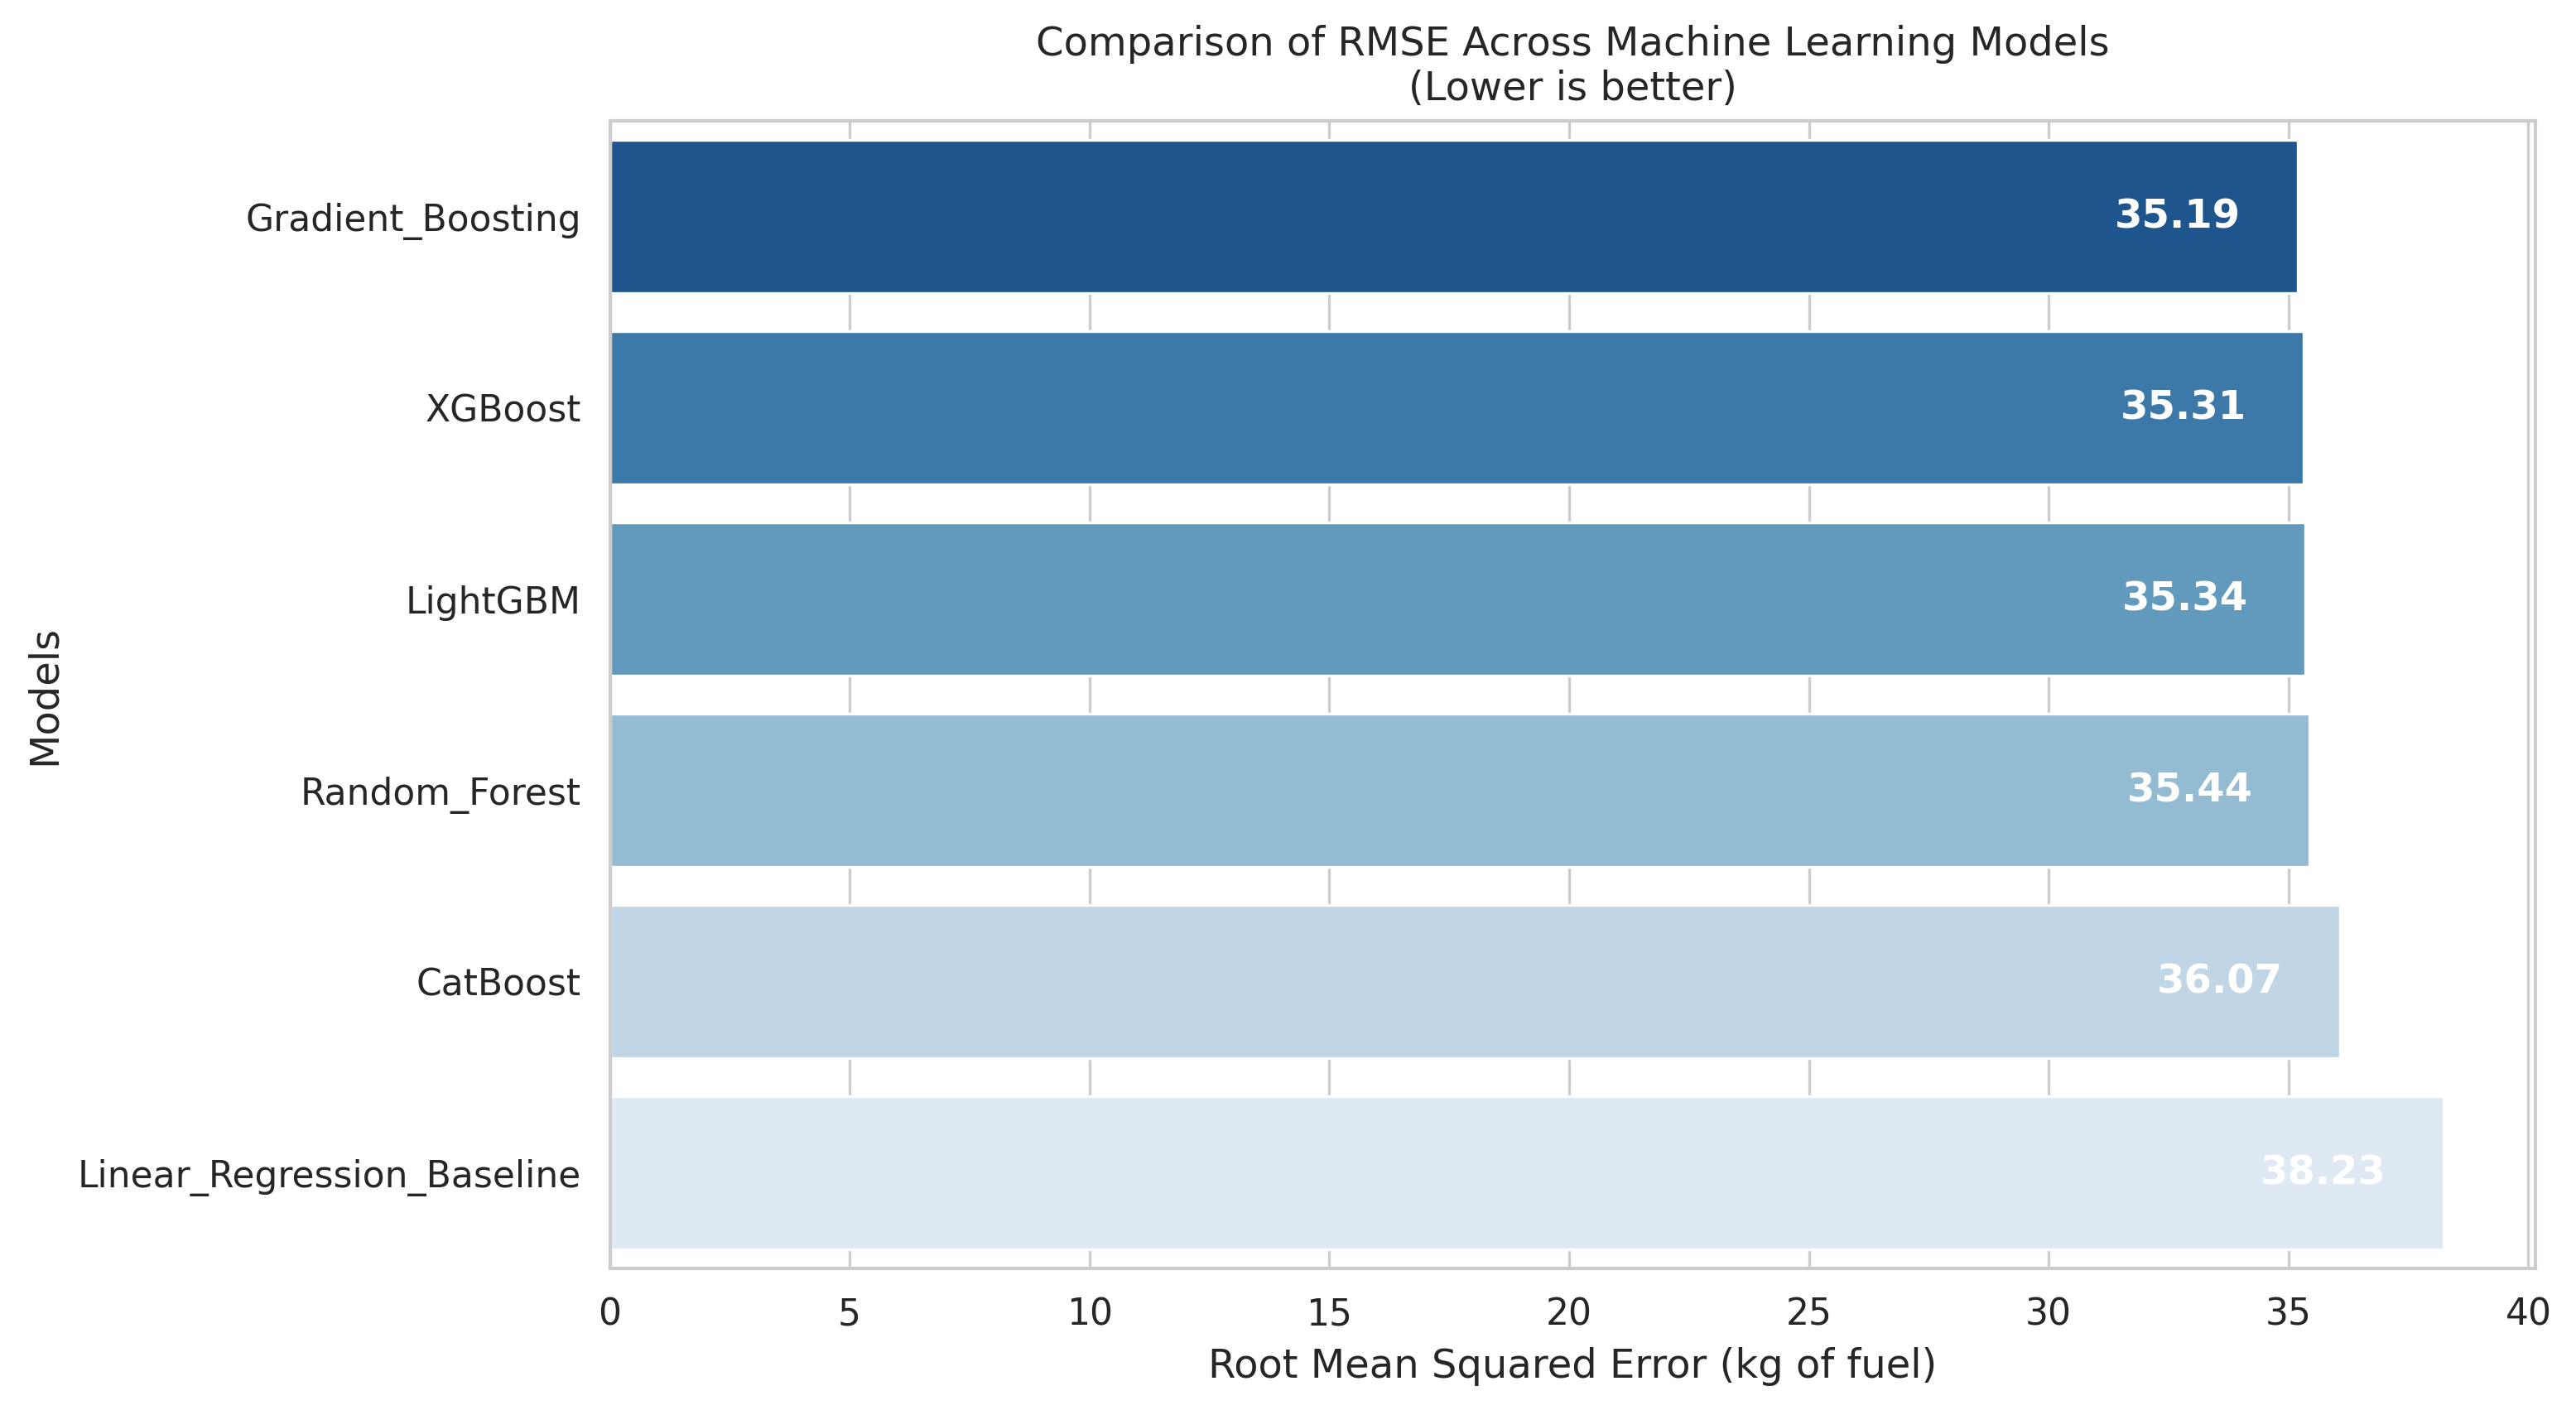
\includegraphics[width=1\linewidth]{images/comparativo_rmse.png}
    \caption{Root Mean Squared Error (RMSE) comparison across the evaluated machine learning models.}
    \label{fig:comparativo_rmse}
\end{figure}

\begin{figure}[htbp]
    \centering
    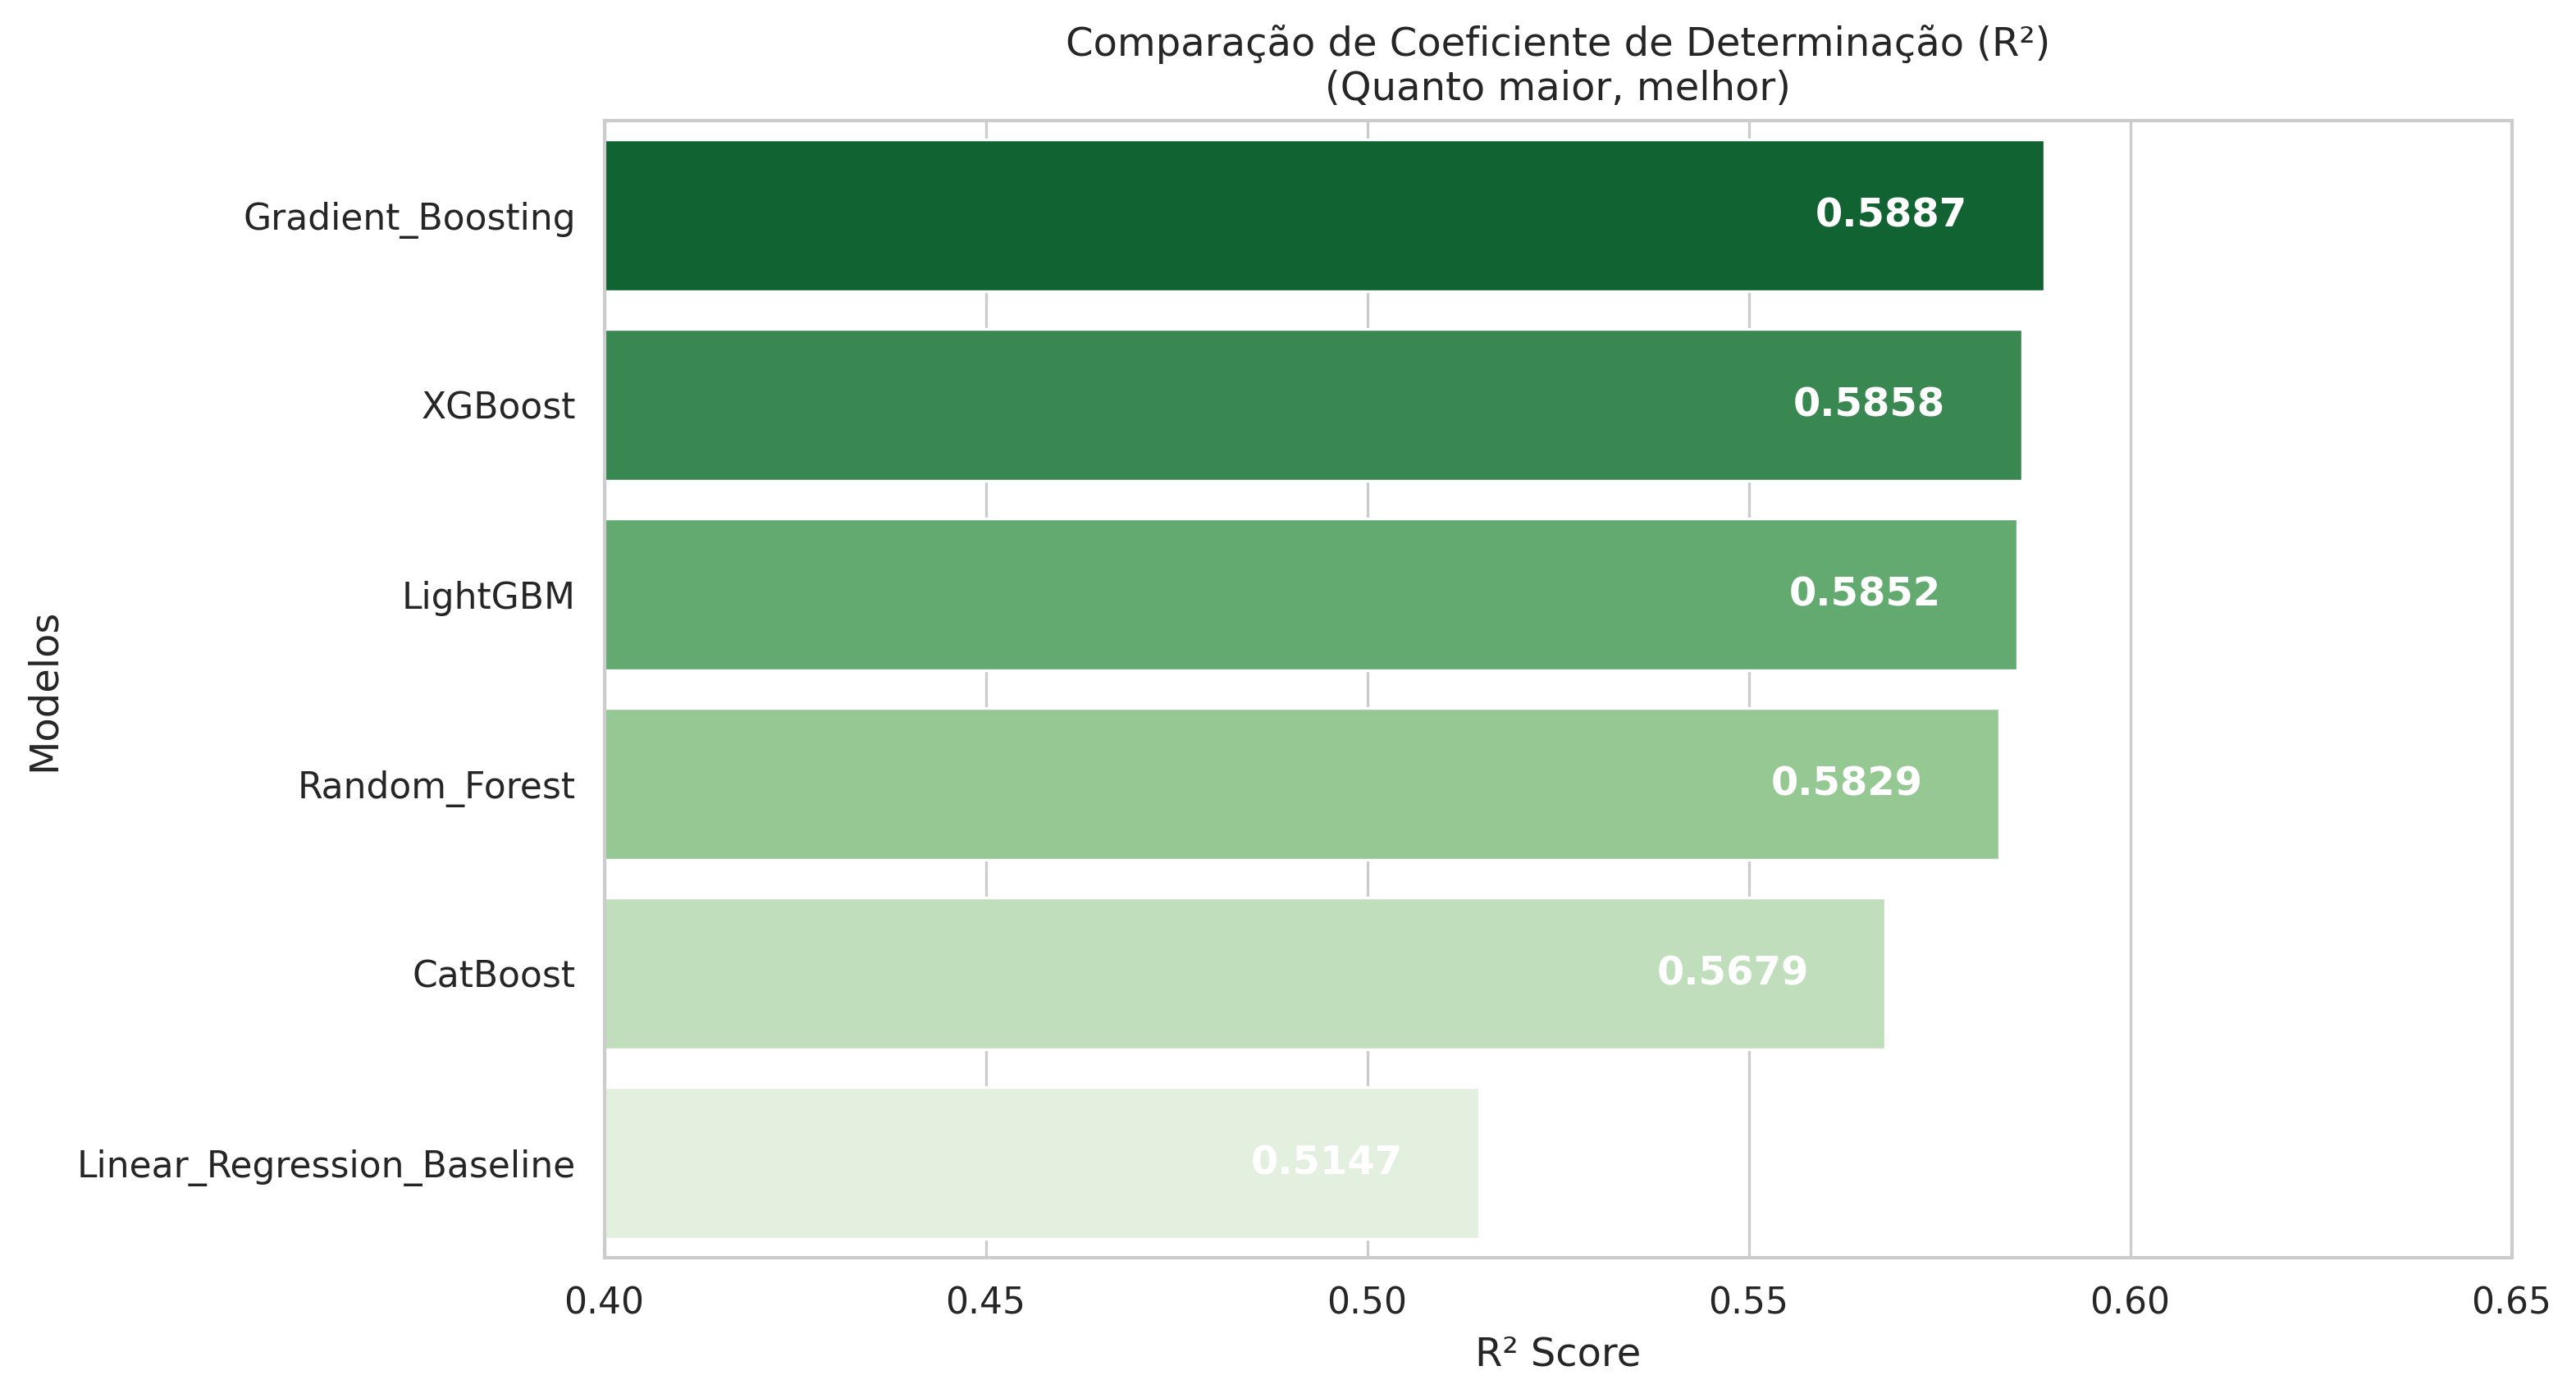
\includegraphics[width=1\linewidth]{images/comparativo_r2.png}
    \caption{Coefficient of Determination ($R^2$) comparison across the evaluated machine learning models.}
    \label{fig:comparativo_r2}
\end{figure}

As observed in Figures \ref{fig:comparativo_rmse} and \ref{fig:comparativo_r2}, all tree-based ensemble methods (Random Forest, Gradient Boosting, XGBoost, LightGBM, and CatBoost) significantly outperformed the Linear Regression baseline, which achieved an $R^2$ of 0.5147 and an RMSE of 38.23 kg. This substantial gap (an improvement of approximately 14\% in $R^2$ variance explained) underscores the highly non-linear nature of air traffic dynamics and the necessity of using advanced algorithms to capture complex interactions between arrival sectors, time of day, and congestion levels.

Among the ensemble methods, the performances were remarkably competitive. The standard Gradient Boosting Regressor (Scikit-Learn implementation) yielded the best overall results, reaching an $R^2$ of 0.5887 and an RMSE of 35.19 kg. It was closely followed by XGBoost and LightGBM. The slightly inferior performance of CatBoost in this specific setup ($R^2$ = 0.5679) can likely be attributed to the fact that we fed it a pre-encoded (One-Hot) dataset to maintain consistency across the benchmark, whereas CatBoost is specifically optimized to internally process native ordinal categorical data.

Overall, explaining nearly 59\% of the variance in additional fuel consumption ($KPI16$) indicates that a substantial portion of its variability can be explained by the selected operational, traffic, and meteorological variables. Predicting tactical fuel penalties prior to TMA entry enables controllers to anticipate bottlenecks and allows airlines to optimize their fuel policies dynamically.

\subsection{Hyperparameter Tuning and Optimization}
Following the baseline evaluation of the machine learning algorithms, an extensive hyperparameter tuning phase was conducted to maximize the predictive capability of the models. The default parameters, while robust, often fail to capture the nuances of complex non-linear relationships present in aviation datasets. This is especially true regarding the trade-off between the learning rate and the number of estimators, and the tendency of tree-based methods to overfit on dominant features such as the predicted transit time (\textit{transit\_tma\_predicted}).

To systematically explore the hyperparameter space, we employed Optuna \cite{akiba2019optuna}, an open-source hyperparameter optimization framework that utilizes Bayesian optimization. Unlike an exhaustive grid search, Optuna's Tree-structured Parzen Estimator (TPE) algorithm probabilistically samples the search space, focusing on regions that are more likely to yield optimal results, thus significantly reducing computational time while improving the search efficiency compared to exhaustive approaches.

\subsubsection{Optimization Strategy}
The tuning process was applied to all applicable tree-based ensemble methods: Random Forest, Gradient Boosting, XGBoost, LightGBM, and CatBoost. For each model, we defined an objective function to minimize the Mean Squared Error (MSE) using a 20\% validation hold-out set. The optimization trials ran iteratively, focusing on the following key aspects:

\begin{itemize}
    \item \textbf{Learning Rate and Estimators Trade-off:} We allowed the framework to explore lower learning rates paired with a higher number of estimators. This combination generally improves the model's ability to converge smoothly to a global minimum without overshooting.
    \item \textbf{Tree Complexity (Depth and Leaves):} The maximum depth of the trees (\textit{max\_depth}) and the maximum number of leaves (\textit{num\_leaves}) were expanded to allow the models to capture deeper, more intricate interactions among the spatial and temporal variables.
    \item \textbf{Regularization (L1/L2 Penalties):} To prevent the models from memorizing the training data, we introduced L1 (\textit{reg\_alpha}) and L2 (\textit{reg\_lambda} or \textit{l2\_leaf\_reg}) regularization terms. This forces the algorithms to keep the tree weights small and generalized.
    \item \textbf{Subsampling and Feature Selection:} We optimized the \textit{subsample} (fraction of rows used per tree) and \textit{colsample\_bytree} (fraction of columns used per tree) parameters. By restricting the models to around 60\% to 80\% of the data or features per iteration, we forced the ensembles to learn from diverse perspectives, reducing their over-reliance on the dominant \textit{transit\_tma\_predicted} feature.
\end{itemize}

\subsubsection{Tuning Results and Winning Model}
The optimization phase yielded substantial improvements across the gradient boosting algorithms, as detailed in Table \ref{tab:tuning_results}.

\begin{table}[htbp]
\caption{Model Performance ($R^2$) Before and After Hyperparameter Tuning}
\label{tab:tuning_results}
\centering
\begin{tabular}{lccc}
\hline
\textbf{Model} & \textbf{Baseline $R^2$} & \textbf{Tuned $R^2$} & \textbf{Improvement} \\
\hline
Linear Regression & 0.5147 & N/A & N/A \\
Random Forest & 0.5829 & 0.5852 & +0.23\% \\
Gradient Boosting & 0.5887 & 0.6212 & +3.25\% \\
LightGBM & 0.5852 & 0.6236 & +3.84\% \\
XGBoost & 0.5858 & 0.6248 & +3.90\% \\
\textbf{CatBoost} & \textbf{0.5679} & \textbf{0.6259} & \textbf{+5.80\%} \\
\hline
\end{tabular}
\end{table}

While the Random Forest algorithm saw only a marginal gain—a behavior that is common in bagging methods which are less sensitive to hyperparameter changes—all gradient boosting architectures experienced significant leaps in performance.

The most notable outcome of the tuning process was the performance of CatBoost. In the baseline evaluation, CatBoost placed last among the tree-based methods ($R^2$ = 0.5679), primarily because the dataset had been pre-processed with One-Hot Encoding to ensure a strict one-to-one benchmark against the other models, whereas CatBoost is natively optimized to handle raw categorical data internally. However, after undergoing Bayesian optimization with Optuna, CatBoost experienced a massive 5.80\% improvement in explained variance, jumping to the first position with an $R^2$ of 0.6259 and an RMSE of 33.56 kg.

These results solidify CatBoost as the winning model of this study. This dramatic leap in performance was heavily driven by the optimization of its specific hyperparameters. First, the number of \textit{iterations} was elevated to 900, coupled with a highly calibrated \textit{learning\_rate} of approximately 0.0596, allowing for steady convergence. The \textit{depth} of the oblivious trees was increased to 9, giving the model the ability to detect deeper conditional patterns without excessive branching. To prevent this increased depth from overfitting, the \textit{subsample} ratio was reduced to 0.734 (meaning each tree was trained on only ~73\% of the data) and the \textit{l2\_leaf\_reg} (L2 regularization coefficient) was refined. These optimized parameters allowed CatBoost to effectively navigate the complex categorical interactions (such as the relationship between specific departure airports and entry sectors) and deliver the most accurate estimations of additional fuel consumption in the Terminal Maneuvering Area.

\subsection{Feature Importance Analysis}
In predictive modeling for air traffic management, understanding the drivers behind a model's decisions is as critical as its overall accuracy. Figure \ref{fig:feature_importance} presents the aggregated feature importance extracted from the best-performing model, the tuned CatBoost regressor. Because the dataset was one-hot encoded, the importances of the dummy variables were aggregated by their base feature name to reflect the true weight of each categorical variable.

\begin{figure}[htbp]
    \centering
    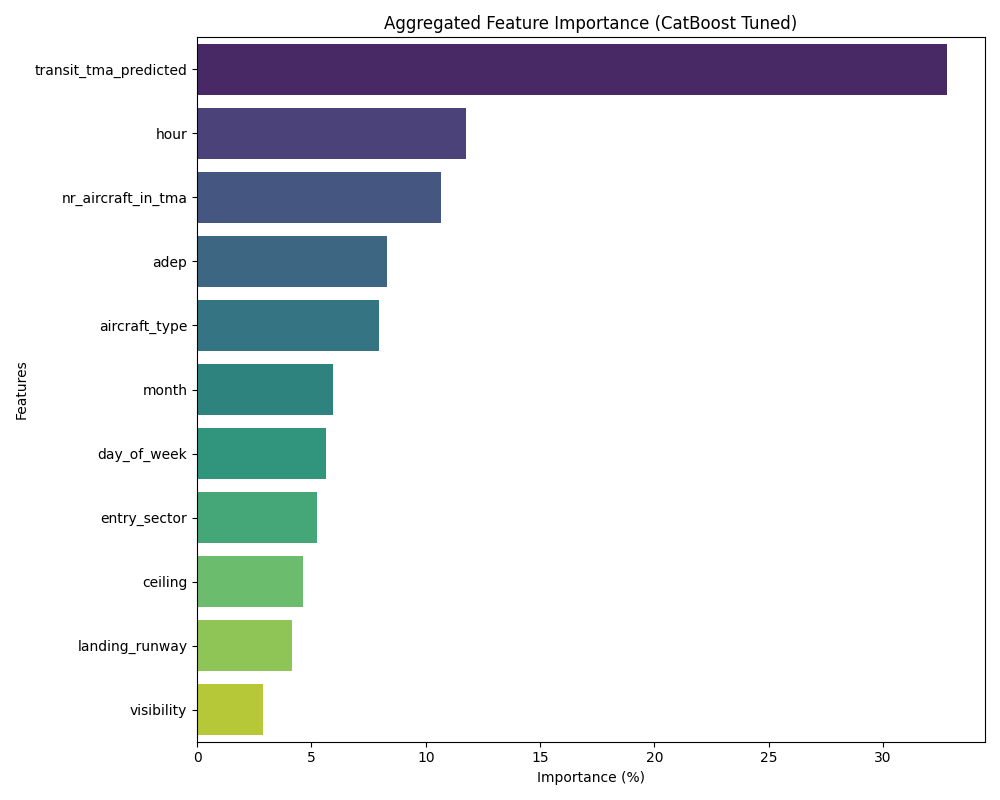
\includegraphics[width=1\linewidth]{images/feature_importance.png}
    \caption{Aggregated feature importance ranking from the tuned CatBoost model.}
    \label{fig:feature_importance}
\end{figure}

The analysis reveals that the moving average of predicted transit time in the TMA (\texttt{transit\_tma\_predicted}) is the most critical explanatory variable, accounting for nearly a third of the model's total predictive power. This outcome underscores the profound impact of airspace congestion on fuel consumption. By effectively tracking the historical density of approaching flights, this engineered feature captures operational conditions that may be associated with delays, holding patterns, or vectoring.

Following the transit time predictor, variables linked to air traffic schedules and volume—specifically the hour of the day (\texttt{hour}) and the concurrent number of aircraft in the TMA (\texttt{nr\_aircraft\_in\_tma})—demonstrate significant importance. These factors are likely associated with controller workload, traffic complexity and the likelihood of experiencing tactical delays upon arrival. Furthermore, the departure airport (\texttt{adep}) and aircraft type (\texttt{aircraft\_type}) hold considerable weight, as different origins imply distinct entry routes and sequencing challenges, while aircraft models inherently possess varied fuel flow capabilities and descent profiles.

Conversely, variables such as cloud ceiling (\texttt{ceiling}), validated landing runway (\texttt{landing\_runway}), and visibility (\texttt{visibility}) showed lower relative importance. While adverse meteorological conditions and runway configurations prompt Air Traffic Control to enforce greater separation minimums, the resulting delays are already largely captured by the primary traffic density metrics, mitigating their direct impact in the model.
